\documentclass[11pt,a4paper]{article}
\usepackage[T1]{fontenc}
\usepackage{lmodern,amsmath,amssymb,amsthm,booktabs,graphicx}
\usepackage[a4paper,top=24mm,bottom=24mm,left=29mm,right=29mm]{geometry}
\usepackage{color}
\definecolor{referenceblue}{rgb}{0.12,0.23,0.40}
\usepackage[colorlinks=true,allcolors=referenceblue]{hyperref}
\hypersetup{pdftitle={Substitution bounds for the inducibility of six-vertex graphs},pdfauthor={Oleg Kyzlasov},pdfsubject={Extremal graph theory},pdfkeywords={inducibility, Petersen graph, rook graph, graph substitution, flag algebras}}
\urlstyle{same}
\newtheorem{theorem}{Theorem}
\newtheorem{lemma}[theorem]{Lemma}
\newtheorem{corollary}[theorem]{Corollary}
\newcommand{\F}{F_{26}}
\newcommand{\BH}{\mathcal H}
\newcommand{\E}{\mathbb E}
\newcommand{\one}{\mathbf 1}
\newcommand{\trans}{\mathsf T}
\DeclareMathOperator{\tr}{tr}
\DeclareMathOperator{\Aut}{Aut}
\setlength{\emergencystretch}{1em}
\setlength{\abovedisplayskip}{8pt plus 2pt minus 2pt}
\setlength{\belowdisplayskip}{8pt plus 2pt minus 2pt}
\setcounter{tocdepth}{1}
\raggedbottom
\title{\bfseries Substitution bounds for the inducibility\\of six-vertex graphs}
\author{Oleg Kyzlasov}
\date{22 November 2026 \quad $\cdot$ \quad Version 2.0}

\begin{document}
\maketitle
\begin{abstract}
Balanced substitutions of the Petersen graph give induced density \(480/11111\)
for the tree \(F_{26}\). This value is sharp among graphs with no induced bull
or house, and lies within \(3.471\cdot10^{-8}\) of a certified unrestricted upper
bound. For \(F_{74}\) we prove a finite counting inequality for substitutions
into the complement of the \(3\)-by-\(3\) rook graph. Equality characterizes
the balanced powers of this graph, with limiting density \(360/7381\).
A rational upper certificate places the unrestricted maximum within
\(6.95\cdot10^{-9}\) of that value. For \(F_{22},F_{29},F_{34}\) and \(F_{62}\)
we give explicit constructions exceeding the values in four conjectures of
Bodn\'ar, Gao, Le\'on, Liu, Pikhurko and Sun (arXiv:2606.00290v3).
For \(F_{29}\), a graph on 36 vertices suffices to define the blowup.
\end{abstract}

\section{Induced density and the Petersen bounds}
The graph \(F=F_{26}\) has vertex set \(\{0,1,2,3,4,5\}\) and edge set
\(\{01,02,05,13,45\}\), where \(ij\) denotes the unordered pair \(\{i,j\}\).
This labelling numbers the vertices clockwise from the top in row 26 of
\href{https://arxiv.org/html/2606.00290v3#S5.T3}{Table~3} of
Bodn\'ar, Gao, Le\'on, Liu, Pikhurko and Sun~\cite{six}. Throughout,
the subscript in \(F_i\) is the index in their catalogue. Each of the
six targets considered here has six vertices. The graphs in which
we count copies can have any order. In particular, the Petersen graph
on ten vertices and the board graph on nine vertices serve as
substitution templates for \(F_{26}\) and \(F_{74}\), respectively.

All finite graphs are simple and undirected. For a graph \(H\) on \(h\)
vertices, let \(c_H(G)\) count the \(h\)-element sets \(A\subseteq V(G)\)
such that \(G[A]\cong H\). Its induced density and inducibility are
\[
 p(H,G)=\frac{c_H(G)}{\binom{|V(G)|}{h}},\qquad
 \lambda_H=\lim_{n\to\infty}\ \max_{|V(G)|=n}p(H,G).
\]
The density is defined for \(|V(G)|\ge h\). The maximum is nonincreasing in \(n\) by averaging over vertex deletions~\cite{pg}. Restricting the maximum to a class closed under induced subgraphs gives its inducibility limit by the same argument, provided the class has graphs of every order.


This paper extends the Petersen case of the first version~\cite{first}.
Sections~\ref{sec:construction} through~\ref{sec:upper} give its construction,
finite extremal theorem and upper certificate. Section~\ref{sec:rook}
proves the corresponding weight inequality for the rook substitution.
Sections~\ref{sec:cycle} and~\ref{sec:perturb} examine four proposed
values from Section~4 of~\cite{six}. All graph numbers and comparisons
in this paper refer to the third arXiv version of that article.

\begin{theorem}\label{th:global}
The unrestricted inducibility satisfies
\begin{equation}\label{eq:interval}
 L:=\frac{480}{11111}
 \ \le\ \lambda_F\ \le\
 U:=\frac{233973195106737927117969229}{5415987671873538702683668480}.
\end{equation}
\end{theorem}

To ten decimal places the lower endpoint is \(0.0432004320\).
Table~3 of~\cite{six}, version~3, lists \(0.0293174175\) and \(0.0432004682\) in this row. The relative increase over the displayed lower value is approximately \(47.35415\%\). Section~5 of~\cite{six} describes the upper entry as numerical output from the order-eight semidefinite program. Here \(U=0.0432004667074510\ldots\) follows from integer Gram factors on eight and nine vertices. The difference \(U-L=3.4703130969\ldots\cdot10^{-8}\) leaves the unrestricted value undetermined by these bounds.

Let \(\BH\) be the class of graphs with no induced bull and no induced house. A bull consists of a triangle with a pendant edge at each of two distinct triangle vertices. A house is the complement of the five-vertex path. Let \(P\) be the Petersen graph and \(P^0=K_1\) the one-vertex graph. Form \(P^{t+1}\) by replacing each vertex of \(P\) by a copy of \(P^t\), putting all possible edges between two copies precisely when the corresponding vertices of \(P\) are adjacent.

\begin{theorem}\label{th:finite}
The inducibility of \(F\) in \(\BH\) is \(L\). For \(G\in\BH\) with \(n\ge1\) vertices,
\begin{equation}\label{eq:finite}
 c_F(G)\le \frac{2(n^6-n)}{33333}.
\end{equation}
Equality holds if and only if \(n=10^t\) and \(G\cong P^t\), for an integer \(t\ge0\).
\end{theorem}

Between successive powers of ten, \eqref{eq:finite} gives an upper estimate for the finite maximum. The proof of the bound uses vertex weights, but the count in \(P^t\) is elementary.

\section{Counting in Petersen substitutions}\label{sec:construction}

\begin{figure}[htb]
\centering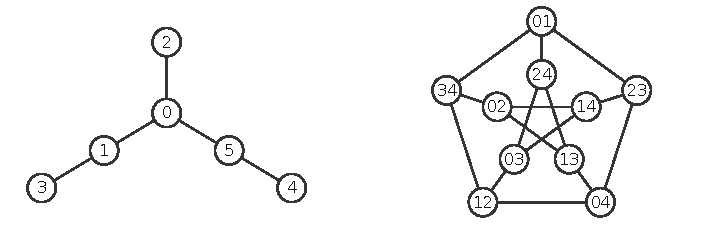
\includegraphics[width=.84\linewidth]{graphs.pdf}
\caption{The tree \(F\) and the Petersen graph \(P\). In \(P\) a vertex \(ij\) represents a two-element subset of \(\{0,1,2,3,4\}\). Two vertices are adjacent when their subsets are disjoint.}
\label{fig:graphs}
\end{figure}

A \emph{module} is a set \(M\) such that each vertex outside \(M\) is joined to all or none of \(M\). A graph is \emph{prime} if it has no module of size between two and its order minus one. In a connected tree a proper module \(M\) of size at least two has an outside neighbour adjacent to all of \(M\). An internal edge would give a triangle, and two outside neighbours would give a four-cycle. Thus the vertices of \(M\) are leaves with a common neighbour. In \(F\) the three leaves have distinct neighbours. In particular, \(F\) is prime.

There are exactly 60 induced copies of \(F\) in \(P\). To see this, fix the centre \(01\). Its three neighbours are the pairs in \(\{2,3,4\}\), and all three must occur. Choose two of them to carry the longer arms. Each has two possible terminal vertices of the form \(\{\epsilon,j\}\), where \(j\) is the omitted element of \(\{2,3,4\}\) and \(\epsilon\in\{0,1\}\). The two terminals have distinct \(j\)'s. They are nonadjacent precisely when they have the same \(\epsilon\). This gives \(3\cdot2=6\) copies per centre. The ten vertices are equivalent, and a copy has exactly one centre.

Put \(n_t=10^t\), \(a_t=c_F(P^t)\). A copy of \(F\) crossing two or more parts takes at most one vertex from each part, since otherwise its intersection with a repeated part would be a proper module. Consequently
\[
 a_0=0,\qquad a_{t+1}=10a_t+60n_t^6,\qquad
 a_t=\frac{60(n_t^6-n_t)}{10^6-10}=\frac{2(n_t^6-n_t)}{33333}.
\]
It follows that \(p(F,P^t)\to 6!\cdot60/(10^6-10)=L\). The house is prime because the five-vertex path is prime and complementation preserves modules. For the bull, none of its 25 subsets of sizes two through four is a module. The same transversal-copy argument now shows that substitution preserves \(\BH\). Since \(P\) is triangle-free, \(P\in\BH\) and hence \(P^t\in\BH\) for every \(t\). Triangles already occur in \(P^2\): an edge inside one part and a single vertex in an adjacent part form one.

\section{A weighted inequality and the hereditary class}\label{sec:restricted}

Give each vertex \(v\) of \(G\) a weight \(x_v\ge0\), with \(\sum_v x_v=1\). Put
\begin{equation}\label{eq:defq}
 q(G,x)=6!\!\sum_{\substack{A\subseteq V(G),\ |A|=6\\G[A]\cong F}}\ \prod_{v\in A}x_v,
 \qquad s_6(x)=\sum_v x_v^6 .
\end{equation}
The first quantity is the probability that six independent draws are distinct and induce \(F\). With uniform weights it is \(6!c_F(G)/|V(G)|^6\). The second is the probability that all six draws coincide. Removing zero-weight vertices leaves both quantities unchanged.

\begin{theorem}\label{th:weighted}
For every finite \(G\in\BH\) and every probability vector \(x\),
\begin{equation}\label{eq:weighted}
 q(G,x)\le L(1-s_6(x)).
\end{equation}
After removal of zero weights, equality holds precisely for the following weighted graphs. Start with one vertex of mass one. A vertex of mass \(y\) may be replaced by a copy of \(P\), giving each of its ten vertices mass \(y/10\) and the former external adjacencies. Perform any finite sequence of these replacements.
\end{theorem}

For triangle-free graphs, Sections~\ref{sec:colour} and~\ref{sec:equality} prove \eqref{eq:weighted} and show that the only positive-support equality examples are \(K_1\) and the equally weighted \(P\). We deduce the full statement by induction.

\begin{proof}[Deduction of Theorem~\ref{th:weighted} from its triangle-free case]
Take positive weights and induct on the number of vertices. For one vertex, both sides of \eqref{eq:weighted} vanish. In a disconnected graph with components \(G_i\), masses \(y_i\) and normalized component weights \(x_i\), connectivity of \(F\) gives \(q(G,x)=\sum_i y_i^6q(G_i,x_i)\). The induction hypothesis bounds this sum by \(L(\sum_i y_i^6-s_6(x))\), strictly below the right side of \eqref{eq:weighted}.

For connected \(G\in\BH\), \href{https://arxiv.org/html/2604.27594v3#S1.Thmtheorem3}{Theorem~1.3} of Belavadi and Ho\`ang~\cite{bh} gives three possibilities. The graph has a nontrivial proper module (a homogeneous set in their terminology), is triangle-free, or has bipartite complement. Lemmas~\ref{lem:tf} and~\ref{lem:equality} cover the triangle-free case. A graph with bipartite complement is the union of two cliques on disjoint vertex sets, with arbitrary edges between them. Its independence number is at most two, whereas the three leaves of \(F\) are independent. Here \(q=0\) and equality forces one positive vertex.

For a nontrivial proper module \(M\) of mass \(y\), contract \(M\) to a vertex of weight \(y\), obtaining \((G/M,x')\). Keeping any one vertex of \(M\) gives an induced copy of the quotient, so both it and \(G[M]\) lie in \(\BH\). By primeness, every copy of \(F\) either lies in \(M\), meets \(M\) once, or avoids \(M\). Write \(x|_M/y=(x_v/y)_{v\in M}\) for the normalized weights on \(M\). Summing over the choice of a vertex in \(M\) gives
\begin{equation}\label{eq:subst}
 q(G,x)=q(G/M,x')+y^6 q(G[M],x|_M/y).
\end{equation}
Since \(s_6(x')=s_6(x)-\sum_{v\in M}x_v^6+y^6\), the two inductive bounds yield \eqref{eq:weighted}. The deficit \(L(1-s_6)-q\) is the quotient deficit plus \(y^6\) times the internal deficit. Equality forces equality in both smaller graphs. Replacing the contracted leaf by the internal substitution tree gives the stated construction. Conversely, the equally weighted \(P\) has \(q=27/625\) and \(s_6=10^{-5}\), hence equality. Equation~\eqref{eq:subst} preserves equality at every replacement.
\end{proof}

With \(x_v=1/n\), \eqref{eq:weighted} gives \eqref{eq:finite}. A leaf at depth \(d\) in the substitution tree has mass \(10^{-d}\). Thus uniform leaf weights force a common depth \(t\) and give \(P^t\) up to isomorphism. Section~\ref{sec:construction} proves attainment at all these orders. Dividing \eqref{eq:finite} by \(\binom n6\) and taking the limit proves Theorem~\ref{th:finite}.

\section{The triangle-free certificate}\label{sec:colour}

\begin{lemma}\label{lem:tf}
Inequality \eqref{eq:weighted} holds for every finite triangle-free graph \(T\) and every nonnegative weight vector of sum one.
\end{lemma}

Sample eight independent vertices of \(T\) with law \(x\). Give each pair of sample positions one of three colours: blue for equal vertices, red for adjacent vertices, white otherwise. Each blue class represents one sampled vertex. Between two classes all pairs have the same colour, and the red quotient is triangle-free. Let \(\mathcal C_n\) consist of all isomorphism types of these coloured patterns on \(n\) positions, allowing any triangle-free quotient. For \(H\in\mathcal C_8\), write \(f_H\) for the number of six-subsets whose red graph is \(F\), and \(b_H\) for the number of all-blue six-subsets. A red copy of \(F\) must use six different classes by primeness. For a random host \(H\) the score
\begin{equation}\label{eq:z}
 z_H=\frac{11111 f_H+480 b_H-13440}{13440}
\end{equation}
therefore has mean \(q(T,x)/L+s_6(x)-1\), since \(\binom86=28\).

A \emph{type} \(\sigma\) is a coloured pattern on \(k\in\{0,2,4,6\}\) positions with a fixed ordering of its vertices, called roots. We choose one such ordering per isomorphism class. The \(\sigma\)-\emph{flags} used here extend this pattern by \(u=(8-k)/2\) positions. Two flags agree if a colour-preserving isomorphism fixes each root. In an ordering of \(V(H)\) whose first \(k\) positions give \(\sigma\), the next \(u\) and last \(u\) positions give flags \(i,j\). Let \(M_{H,\sigma}(i,j)\) count the orderings giving this pair. Interchanging the two groups shows that \(M_{H,\sigma}\) is symmetric.

For each type the supplement supplies an integer matrix \(B_\sigma\), a rational symmetric matrix \(Q_\sigma\), and a positive divisor \(d_\sigma\). We write \(\tr\) for trace, \({}^{\trans}\) for transpose, and \(Q\succ0\) for positive definiteness. The certificate gives
\begin{equation}\label{eq:row}
 z_H+\sum_\sigma \frac{\tr(M_{H,\sigma}B_\sigma Q_\sigma B_\sigma^{\trans})}{d_\sigma}\le0
 \quad(H\in\mathcal C_8),\qquad Q_\sigma\succ0 .
\end{equation}
The rows of \(B_\sigma\) are indexed by flags. A coloured host is determined by its triangle-free quotient and its positive class sizes, up to automorphisms of the quotient. To check the quotient catalogue, add a vertex with each possible independent neighbourhood and compare the resulting labelled counts with the sum of the orbit sizes. Burnside's lemma then counts the orbits of class sizes. The verifier reconstructs the colour masks and tests that distinct entries represent distinct orbits. For orders one through eight the catalogue sizes are
\[
   1,\quad 3,\quad 6,\quad 17,\quad 41,\quad 125,\quad 388,\quad 1491 .
\]
Root subsets, their label-preserving embeddings and the two complementary extensions give an independent recount of every product coefficient. In packed symmetric storage, a diagonal coefficient is \(M_{ii}\), and an off-diagonal one is \(2M_{ij}\). For each block the checker forms \(R_\sigma=Q_\sigma-C_\sigma C_\sigma^{\trans}\) using the supplied rational factor \(C_\sigma\). In each row \(R_{ii}>\sum_{j\ne i}|R_{ij}|\), so \(R_\sigma\) and \(Q_\sigma\) are positive definite. Expanding \(B_\sigma Q_\sigma B_\sigma^{\trans}\) and substituting in \eqref{eq:row} checks 1,491 inequalities in 146 blocks of total \(Q\)-dimension 4,164. Exactly 276 host inequalities are tight.

\begin{proof}[Proof of Lemma~\ref{lem:tf}]
Condition on the vertices drawn at the first \(k\) positions. If they give the labelled type \(\sigma\), let \(p_\sigma\) be the conditional probability vector for one extension. Otherwise put \(p_\sigma=0\). The two groups of \(u\) new draws are conditionally independent and identically distributed. Exchangeability gives
\[
 \E M_{H,\sigma}=8!\,\E[\one_\sigma p_\sigma p_\sigma^{\trans}].
\]
Here \(\one_\sigma\) is the indicator of a root match. With \(w=B_\sigma^{\trans}p_\sigma\), the expected trace in \eqref{eq:row} is \(8!\,\E[\one_\sigma w^{\trans}Q_\sigma w]\ge0\). Taking expectations gives \(\E z_H\le0\), hence \eqref{eq:weighted} for every finite triangle-free \(T\) and every probability vector \(x\).
\end{proof}

\section{Equality in the triangle-free inequality}\label{sec:equality}

\begin{lemma}\label{lem:equality}
If all weights are positive, equality in Lemma~\ref{lem:tf} holds precisely for one vertex or for the Petersen graph with all weights \(1/10\).
\end{lemma}

\begin{proof}
If \(q=0\), equality gives \(s_6=1\) and the support has one vertex. Suppose \(q>0\). An \emph{anchor} is a copy of \(F\) ordered to match the six-root type used in the certificate (block 142, counting from zero). This type has 28 one-vertex flags. Row reduction modulo the prime \(1000000007\) gives 27 pivots in its \(28\)-by-\(27\) integer matrix \(B\), so \(B\) has rank 27 over \(\mathbb R\). Fix the anchor \(R=(01,02,12,03,13,24)\) in \(P\), using the vertex names in Figure~\ref{fig:graphs}. Each of the ten vertices of \(P\) gives a different flag over \(R\). Let \(v\) be the indicator vector of those ten flags. Direct multiplication gives \(B^{\trans}v=0\), so \(\ker B^{\trans}=\mathbb R v\).

At equality every nonnegative expected quadratic form in \eqref{eq:row} vanishes. Since the support is finite and all weights are positive, each fixed anchor has positive probability. Positive definiteness of its \(Q\) gives \(B^{\trans}p=0\) for its one-extension distribution \(p\). Its entries sum to one, hence \(p=v/10\). Six flags are coincidences with the roots, so every vertex belonging to an induced \(F\) has mass \(1/10\). Each of the other four flags prescribes a red neighbourhood on the roots and has total mass \(1/10\).

Number the positions of \(R\) from zero. Table~\ref{tab:profiles} gives, for each outside vertex of \(P\), a root whose replacement yields another induced copy of \(F\). This test uses only adjacencies to the anchor. It therefore applies to any vertex with the same profile in \(T\). Each such vertex has weight \(1/10\), so each of the four classes is a singleton.

\begin{table}[htb]
\centering
\begin{tabular}{ccl}
\toprule
Vertex of \(P\) & Neighbour positions in \(R\) & Position to replace\\
\midrule
\(04\) & \(\{2,4\}\) & \(3\)\\
\(14\) & \(\{1,3\}\) & \(4\)\\
\(23\) & \(\{0\}\)   & \(2\)\\
\(34\) & \(\{0,1,2\}\) & \(5\)\\
\bottomrule
\end{tabular}
\caption{The four external profiles of a Petersen anchor and witnesses for the replacement step.}\label{tab:profiles}
\end{table}

The support now has ten equally weighted vertices. Only the six pairs among the outside vertices are undecided. Of the 64 completions, seven are triangle-free. Their numbers of induced copies, with multiplicities, are \(26,34,38,38,44,44,60\). The unique completion with 60 copies is \(P\). Equality requires exactly 60 since \(q=720c_F/10^6\) and \(s_6=10^{-5}\). The converse follows from the count in Section~\ref{sec:construction}.
\end{proof}

\section{The unrestricted upper certificate}\label{sec:upper}

For ordinary simple graphs, we combine an eight-vertex score with one nine-vertex term. Both are built from positive semidefinite quadratic forms in flags with common roots~\cite{raz}.

Let \(s_0=2^{42}\). For 169 types \(\sigma\) of sizes \(k=2,4,6\), the data specify an integer matrix \(A_\sigma\) and a map classifying extensions by \(u=(8-k)/2\) vertices. Each map is invariant under permutations of the added vertices. Put \(K_\sigma=A_\sigma A_\sigma^{\trans}/s_0^2\). For an eight-vertex graph \(H\) let
\[
 s(H)=p(F,H)+\frac1{8!}\sum_{\pi,\sigma}
       \one_\sigma(\pi) K_\sigma(i_\pi,j_\pi).
\]
Here \(\pi\) orders \(V(H)\). The two flag indices refer to the first and second groups after the roots. A root mismatch contributes zero.
For a nine-vertex graph \(J\), put
\begin{equation}\label{eq:nine}
 t(J)=\frac19\sum_{v\in V(J)}s(J-v)
  +\frac1{630}\sum_{r,S} K_1\big(i(r,S),\,i(r,S^{c})\big).
\end{equation}
In the last sum \(r\) is one labelled root, \(S\) ranges over four-subsets of the other eight vertices, and \(S^c=V(J)\setminus(S\cup\{r\})\). There are \(9\binom84=630\) choices. The index \(i(r,S)\) classifies the graph induced by \(\{r\}\cup S\) with \(r\) distinguished. It takes 90 values and \(K_1=A_1A_1^{\trans}/s_0^2\) for the supplied integer matrix \(A_1\). On nine-vertex graphs, \(\max_J t(J)=U\).

\begin{proof}[Proof of the upper bound in Theorem~\ref{th:global}]
Draw nine vertices independently and uniformly from an \(n\)-vertex graph \(G\), \(n\ge6\). Join two sample positions if their underlying vertices are adjacent. Conditional on the underlying roots, the two extensions are independent with the same distribution \(p\). For each matching type the conditional mean of its Gram entry is \(p^{\trans}Kp\ge0\). A root mismatch contributes zero. An induced copy of \(F\) uses six distinct underlying vertices by primeness. Thus the mean density term is \(6!c_F(G)/n^6\), and
\[
 \frac{(n)_6}{n^6}\,p(F,G)\le \E t(J)\le U,\qquad
 (n)_6=n(n-1)\cdots(n-5).
\]
The prefactor tends to one. Maximizing over \(G\) and taking the limit proves the bound.
\end{proof}

The verifier forms the integer Gram products, tests the classifier symmetries, recounts the induced copies and evaluates \(s(H)\) on all \(8!\) vertex orderings. For \eqref{eq:nine} it verifies every deletion and enumerates each five-subset with each choice of root. The common denominator of the nine-vertex scores is \(9\cdot8!\,s_0^2\). Canonical forms distinguish the catalogue entries. The number of vertex orders giving a canonical form is the size of the automorphism group \(\Aut(J)\). For \(n=8,9\), the sums \(\sum_J n!/|\Aut(J)|\) over the respective catalogues equal \(2^{28}\) and \(2^{36}\), accounting for every labelled graph. The catalogues have 12,346 and 274,668 entries. Their exact scores give the upper endpoint of \eqref{eq:interval}.

\section{A sharp bound for rook substitutions}\label{sec:rook}

Let \(H=F_{74}\) have edges \(01,03,04,12,13,35,45\) on
\(\{0,\ldots,5\}\). Index the cells of a \(3\)-by-\(3\) board by
\((a,b)\in\{0,1,2\}^2\). In the graph \(R\), two cells are adjacent
when their row indices differ and their column indices differ. Thus \(R\)
is the complement of the rook graph. Figure~\ref{fig:rook} exhibits one
induced copy of \(H\) in \(R\). A finite \emph{rook substitution}
is either a single vertex or a substitution into \(R\) of nine nonempty
rook substitutions. The nine graphs may have different orders and depths.
Write \(R^k\) for the result when every branch has depth \(k\), with
\(R^0=K_1\) and \(|V(R^k)|=9^k\).

\begin{figure}[htb]
\centering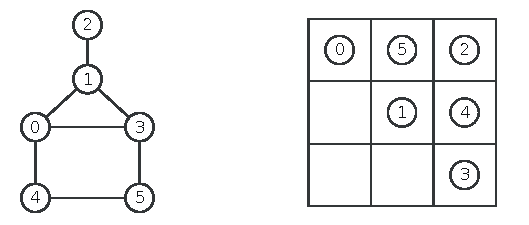
\includegraphics[width=.70\linewidth]{rook-example.pdf}
\caption{An induced copy of \(F_{74}\) in the nine-cell template.
Each vertex on the left occupies the cell with the same label on the
right. Two numbered cells are adjacent exactly when they lie in
different rows and different columns. The three blank cells are the
remaining vertices of the template.}
\label{fig:rook}
\end{figure}

\begin{theorem}\label{th:rook}
For a rook substitution \(G\) of order \(n\ge1\),
\[
 c_H(G)\le \frac{36(n^6-n)}{9^6-9}.
\]
Equality holds precisely for \(R^k\), \(k\ge0\). The largest limiting
density along these substitutions is \(D=360/7381\). For arbitrary
graphs the following rational bounds hold:
\[
 D\le\lambda_H\le
 U_R:=\frac{11321089900811290113624899}{232113757366008801543585792}.
\]
\end{theorem}

Row 74 of Table~3 of~\cite{six} gives \(0.0260416809\) as its lower
entry and \(0.0487738848\) as its numerical upper entry.
Here \(D=0.0487738788782\ldots\) and \(U_R-D<6.95\cdot10^{-9}\).
The rational upper bound is slightly larger than the published numerical
entry. It supplies an independently checkable endpoint.

Let \(\mathcal S\) be the six-subsets of the board inducing \(H\).
There are \(36\) such sets. This count takes only \(\binom96=84\)
tests: form the adjacency matrix on each set and compare it with the
permutations of the displayed edge list. A second finite test establishes
that \(H\) is prime: for each of its \(56\) subsets of sizes two through
five there is an outside vertex joined to some but not all of the subset.
Thus a copy meeting several children of a substitution uses six distinct
children.

\begin{lemma}\label{lem:rook}
For nonnegative cell masses \(x_0,\ldots,x_8\) of total mass one,
\[
 720\sum_{S\in\mathcal S}\prod_{v\in S}x_v
 \ \le\ D\left(1-\sum_{v=0}^{8}x_v^6\right).
\]
Equality holds at the uniform vector and at the nine vectors supported
on a single cell, and nowhere else.
\end{lemma}

\begin{proof}
We give the integer coefficient certificate. In an ordering \(\pi\) with
\(x_{\pi(0)}\le\cdots\le x_{\pi(8)}\), set
\(x_{\pi(j)}=d_0+\cdots+d_j\). All \(d_j\) are nonnegative.
Homogenise the proposed inequality and divide by \(D\). It suffices
to show that every coefficient of
\[
 \left(\sum_v x_v\right)^6-\sum_v x_v^6
       -14762\sum_{S\in\mathcal S}\prod_{v\in S}x_v
\]
is nonnegative in the variables \(d_j\), since \(720/D=14762\).
Index a monomial by a nondecreasing tuple \(t=(t_1,\ldots,t_6)\);
put \(m(t)=6!/\prod_j |\{i:t_i=j\}|!\).
The coefficient from the first two terms is
\[
 m(t)\left(\prod_{i=1}^6(9-t_i)-(9-t_6)\right).
\]
For the last sum, replace each cell of \(S\) by its rank in \(\pi\).
For each of the six ranks \(h\), choose an integer from \(0\) to \(h\).
Count the choices whose sorted list equals \(t\); sum these counts
over \(S\), and multiply by \(14762\).

Row permutations, column permutations and transposition give a group
of \(72\) board symmetries. Its action on the \(9!\) orderings is free.
The checker visits one ordering per orbit and performs the subtraction
just described for all \(\binom{14}6=3003\) monomials. All
\(5040\cdot3003=15\,135\,120\) differences are nonnegative. In every
ordering the coefficients of \(d_j^6\), \(1\le j\le7\), and of
\(d_0^4d_8^2\) are strictly positive. The full enumeration is specified
by the rank rule above and reproduced by the function
\texttt{rook} in the supplement.

At equality the seven intermediate increments vanish. The last positive
coefficient forces either \(d_8=0\) (all masses equal) or \(d_0=0\)
(one nonzero mass). Substitution gives equality in both cases, using
\(720\cdot36/(9^6-9)=D\).
\end{proof}

\begin{proof}[Proof of Theorem~\ref{th:rook}]
Let the child orders be \(n_0,\ldots,n_8\), with sum \(n\).
Primeness gives the exact count
\[
 c_H(G)=\sum_i c_H(G_i)+\sum_{S\in\mathcal S}\prod_{i\in S} n_i.
\]
Apply the lemma to \(n_i/n\), multiply by \(n^6/720\), and add the
inductive bounds for the children. The terms in \(\sum_i n_i^6\)
cancel, leaving \(D(n^6-n)/720\). Equality requires nine equal
positive orders and equality in every child. Induction from order one
then gives \(G=R^k\) up to isomorphism. Conversely these graphs attain
equality at every depth. Dividing by \(\binom n6\) and letting
\(n=9^k\) tend to infinity proves the limiting assertion.

For the unrestricted upper bound use the eight-vertex score \(s\) of
Section~\ref{sec:upper} with target \(H\), denominator \(2^{40}\), and the
169 integer factors in \texttt{f74/factors.txt}. These factors come
from the \href{https://github.com/bodnalev/supplementary_files/blob/9f356bb3dc10dcacd4d26a4eb1d556c2650e4e1b/graph_inducibility_6vtx/certs/inexact_74.pickle}{numerical certificate for \(F_{74}\)} of~\cite{six}.
For each of the \(12\,346\) eight-vertex hosts, the checker enumerates
its \(8!\) orderings, counts its induced copies of \(H\), and evaluates
the Gram terms. The largest integer numerator is
\(2377428879170370923861228790\) over \(8!\,2^{80}\); their ratio
reduces to \(U_R\). It occurs at host 10609 in the zero-based catalogue
order of the supplement. In particular, this score exceeds \(D\) by
\[
 U_R-D=\frac{11906124963772974494399}{1713231643118510964193206730752}.
\]
The orbit sizes sum to \(2^{28}\). Conditional
independence of the two flag extensions makes each Gram term
nonnegative in expectation, as in the proof of Theorem~\ref{th:global}.
Primeness of \(H\) again excludes repeated vertices in a sampled copy.
Taking the limit bounds \(\lambda_H\) by \(U_R\).
\end{proof}

To state the structural condition precisely, a graphon is a symmetric
measurable function \(W:[0,1]^2\to[0,1]\). Sample a graph by drawing
independent uniform points and, conditional on the points, placing
each edge independently with the probability given by \(W\).
The probability of obtaining \(H\) on \(h=|V(H)|\) points is \(p(H,W)\).
The graph limit theorem gives \(\lambda_H=\max_W p(H,W)\)~\cite{limits}.
Suppose a maximizer admits a measurable partition into nine
positive-measure cells with \(W\) equal almost everywhere on each
between-cell rectangle to the corresponding entry of the adjacency
matrix of \(R\). If the cell masses are \(x_i\)
and the unrestricted maximum is \(t\), the within-cell contributions
sum to at most \(t\sum_i x_i^6\). Lemma~\ref{lem:rook} bounds the rest
by \(D(1-\sum_i x_i^6)\). Then \(t\le D\), since \(\sum_i x_i^6<1\).
Thus a single maximizing graphon with such a partition would give the
unrestricted equality. The coefficient certificate proves the implication
under this partition hypothesis. The unconditional result proved here
is the interval in Theorem~\ref{th:rook}.

\section{A cycle and an isolated vertex}\label{sec:cycle}

Let \(J=F_{29}=C_5\sqcup K_1\). Conjecture~4.7 of~\cite{six} (v3)
gives the value \(24/1555\). Here \(C_5\) is the cycle on five vertices
and \(\sqcup\) denotes disjoint union. Write \(J[J]\) for the graph
obtained by substituting a copy of \(J\) at every vertex of \(J\).
We first give a counterexample whose
verification needs only a count of induced subgraphs of one finite graph.

\begin{theorem}\label{th:cycle}
The balanced independent blowup of the \(36\)-vertex graph \(J[J]\)
has limiting \(J\)-density \(12995/839808>24/1555\).
\end{theorem}

\begin{proof}
Index the six groups by the vertices of \(J\) and place a copy of \(J\)
in each. Between two groups put all edges if their indices are adjacent
in \(J\), and none otherwise. The cycle of an induced \(J\) must
lie in one group or use five distinct groups: \(C_5\) is prime, as is
seen by testing its subsets of sizes two through four.

In the latter case it occupies the five cycle groups. Each of these
is complete to two other occupied groups, so the isolated vertex must
lie in the sixth group. This gives \(6^6\) copies. If the cycle lies in
one group, that group contains exactly one induced \(C_5\). The isolated
vertex can lie in a different, nonadjacent group; there are \(20\)
ordered pairs of distinct nonadjacent groups and six choices of vertex
in the second. Finally, there is one entirely internal copy per group.
The total is \(6^6+20\cdot6+6=46\,782\).

Now replace each of the 36 vertices by an independent set of size \(m\).
Every pair of vertices in \(J\) has a third vertex distinguishing them,
so the six vertices of a copy occupy six different sets. Dividing
\(46\,782\,m^6\) by \(\binom{36m}6\) and passing to the limit gives
\[
 \frac{720\cdot46\,782}{36^6}=\frac{12995}{839808}
 =\frac{24}{1555}+\frac{51833}{1305901440}.
 \qedhere
\]
\end{proof}

A larger bound follows from two disconnected components. Let \(C\)
be the limit of iterated balanced substitutions into \(C_5\).
Equivalently, sample each point as an infinite word on five equiprobable
letters; the first letter at which two words differ determines their
adjacency in \(C_5\). Write \(c=p(C_5,C)\) and \(d=p(J,C)\).
For the cycle there are \(5!\) transversal assignments and five choices
for an entirely internal copy. For \(J\), a transversal cycle leaves
no group for an isolate. An internal cycle and an external isolate
use one of ten ordered nonadjacent pairs of groups; the isolate can
occupy any of the six sample positions. Hence
\[
 c=\frac{120+5c}{5^5}=\frac1{26},\qquad
 d=\frac{60c+5d}{5^6}=\frac3{20306}.
\]
Give two copies of \(C\) masses \(a=167216/10^6\) and \(b=1-a\)
and put no edges between them. The cycle stays in one component, while
the isolate may be in either. This gives the unrestricted lower bound
\begin{equation}\label{eq:cycles}
 \lambda_J\ge d(a^6+b^6)+6c(a^5b+ab^5)
 =\frac{722993599084786863008549024709}{46551227569580078125000000000000}.
\end{equation}
Finite-depth substitutions converge to these densities: the probability
that any two of six sampled words share a prefix of length \(k\) is
at most \(15/5^k\). Component sizes can be chosen in the given rational
ratio by uniform blowups.

\section{Three perturbations of recursive constructions}\label{sec:perturb}

Conjectures 4.5, 4.8 and 4.10 of~\cite{six} give rational values
for \(F_{22}, F_{34}\) and \(F_{62}\), respectively. The effect of changing
one mass parameter is small, so we give finite-depth witnesses and
take all comparisons in rational arithmetic.

\begin{theorem}\label{th:perturb}
\(\lambda_{F_{22}}>1440/23327\), and both
\(\lambda_{F_{34}}\) and \(\lambda_{F_{62}}\) exceed \(5760/88573\).
Each strict inequality already holds for the limiting density of a
blowup of the two-level pattern defined below.
\end{theorem}

Use the graphs and templates in Table~\ref{tab:parts}. A listed pair
of distinct parts is complete, and every other such pair is empty.
A part marked recursive receives a scaled copy of the whole construction.
Of the remaining parts all are independent for \(F_{22}\) and \(F_{34}\),
and all are cliques for \(F_{62}\). These specifications use the edge
lists in the \emph{statements} of the three conjectures in v3.

\begin{table}[htb]
\centering\small
\begin{tabular}{@{}llll@{}}
\toprule
Graph & Edges of the target & Edges between parts & Recursive parts\\
\midrule
\(F_{22}\) & 01 03 04 12 15 & 01 02 13 & 0, 1\\
\(F_{34}\) & 01 02 03 04 12 15 & 01 02 03 04 14 23 24 25 45 & 0, 2, 4\\
\(F_{62}\) & 01 03 04 05 12 13 45 & 01 05 12 14 15 23 24 25 35 & 1, 2, 5\\
\bottomrule
\end{tabular}
\caption{Templates for the perturbations. Part labels start at zero.}
\label{tab:parts}
\end{table}

Let \(r\) count the recursive parts. There are also \(r\) constant parts.
Give each recursive part mass \(x\) and each constant part mass
\(y=1/r-x\), for \(0<x<1/r\).

\begin{proof}
The contribution from six points in at least two parts is
\(A_r(x)=c_r x^2y^4\), with \(c_2=180\) and \(c_3=2160\).
Here is an explicit enumeration for these coefficients. Fix the
labelling of the target in Table~\ref{tab:parts}. Run over the
\((2r)^6\) maps from its vertices to the parts, omitting constant maps.
Discard a map if some required edge or nonedge disagrees with a fixed
bit of the template. In each surviving map exactly two target vertices
use recursive parts and they use different parts. Thus every required
bit is already determined. Multiply the number of surviving maps by
the number of distinct labellings of the target, \(6!/|\Aut(F)|\).
In table order there are \(2,6,6\) surviving maps and \(90,360,360\)
labellings, giving \(180,2160,2160\).
These finite counts are repeated in the supplement by assigning one
vertex at a time and pruning on the first conflicting pair.

Let \(q=rx^6\). Six points in one constant part cannot give any of the
three targets. Six points in one recursive part restart the count.
After two levels, finish all remaining recursive parts by independent
sets. The resulting density is
\[
 B_r(x)=A_r(x)(1+q).
\]
There are \(2r^2+r\) terminal parts. For rational masses this density
is attained in the limit of finite graphs by taking part sizes in those
proportions. Sampling six vertices without replacement and sampling
six independent part labels have the same limit.

For completeness, the infinite recursion has density
\(D_r(x)=A_r(x)/(1-q)\). At \(x_0=1/(3r)\) its values are exactly
the respective conjectured fractions. On \(0<x<1/r\), its derivative
has the sign of \(1-3rx+2rx^6\), which is positive at \(x_0\).
To certify the finite-depth claim, substitute the following rational
choices directly in \(B_r\). The final column gives strict lower
bounds on the difference, with the entries interpreted as exact rationals.
\[
\begin{array}{c c c c}
 r & x & D_r(x_0) & B_r(x)-D_r(x_0)\\
 2 & 166681/10^6 & 1440/23327 & >5/10^{10}\\
 3 & 111112/10^6 & 5760/88573 & >9/10^{12}
\end{array}
\]
Both inequalities follow by clearing the positive denominators. The
supplement also flattens the two levels into a single matrix and
recounts compatible assignments directly with the terminal masses.
\end{proof}


\clearpage
\section*{Verification and data}
The archive \texttt{six-vertex-certificates.zip} contains the data and
source code for the finite calculations. Run \texttt{python -B verify.py}
from its extracted directory. The command checks file hashes, rebuilds
the finite certificates, and compares exact results. All five new
construction counts and the rook weight inequality can also be checked
with \texttt{python -B verify.py --part cases}, using the Python
standard library. The unrestricted upper bounds use a C++20 compiler.
The README gives the data formats, provenance and commands for running
each calculation separately.

The unrestricted calculation for \(F_{26}\) started from the \href{https://github.com/bodnalev/supplementary_files/blob/9f356bb3dc10dcacd4d26a4eb1d556c2650e4e1b/graph_inducibility_6vtx/certs/inexact_26.pickle}{order-eight numerical data for \(F_{26}\)} accompanying~\cite{six}. The supplement gives the revision and checksum.

\begin{thebibliography}{9}
\small\raggedright\setlength{\itemsep}{3pt}
\bibitem{bh} M.~Belavadi and Ch\'inh T.~Ho\`ang.
Structural description of (bull, house)-free graphs.
\href{https://arxiv.org/abs/2604.27594v3}{arXiv:2604.27594v3} (2026), Theorem~1.3.
\bibitem{six} Levente Bodn\'ar, Jun Gao, Jared Le\'on, Xizhi Liu, Oleg Pikhurko and Shumin Sun.
The inducibility of 6-vertex graphs.
\href{https://arxiv.org/abs/2606.00290v3}{arXiv:2606.00290v3} (2026), Sections~4 and~5, Tables~2 and~3.
\href{https://github.com/bodnalev/supplementary_files/tree/9f356bb3dc10dcacd4d26a4eb1d556c2650e4e1b/graph_inducibility_6vtx}{Supplementary data}.
\bibitem{first} O.~Kyzlasov. Petersen substitutions and the inducibility
of the six-vertex tree \(F_{26}\). Zenodo, version 1.0 (2026).
\href{https://doi.org/10.5281/zenodo.24341542}{doi:10.5281/zenodo.24341542}.
\bibitem{limits} L.~Lov\'asz and B.~Szegedy. Limits of dense graph sequences.
\emph{J. Combin. Theory Ser. B} \textbf{96} (2006), 933-957.
\href{https://arxiv.org/abs/math/0408173}{arXiv:math/0408173}.
\bibitem{pg} N.~Pippenger and M.~C.~Golumbic. The inducibility of graphs.
\emph{J. Combin. Theory Ser. B} \textbf{19} (1975), 189-203.
\href{https://doi.org/10.1016/0095-8956(75)90084-2}{doi:10.1016/0095-8956(75)90084-2}.
\bibitem{raz} A.~A.~Razborov. Flag algebras.
\emph{J. Symbolic Logic} \textbf{72} (2007), 1239-1282.
\href{https://doi.org/10.2178/jsl/1203350785}{doi:10.2178/jsl/1203350785}.
\end{thebibliography}
\end{document}
